\documentclass[runningheads]{llncs}
\usepackage[T1]{fontenc}
\usepackage{booktabs}
\usepackage{graphicx}
\usepackage{array}
\usepackage{longtable}
\usepackage{amsmath}
\usepackage{graphicx}
\usepackage{footmisc}
\usepackage{tikz}
\usepackage{color, soul}
\usepackage{multirow}
\usepackage{tabularx}
\usepackage{gensymb}
\usepackage[hyphens]{url}
\usepackage{xurl}
\usepackage{rotating}
\usepackage{caption}
\usepackage{booktabs}
\usepackage{titlesec}
\usepackage[euler]{textgreek}
\usetikzlibrary{positioning,arrows.meta,shapes.misc, fit}
\usepackage[numbers]{natbib}
\usepackage[colorlinks=true, allcolors=blue]{hyperref}
\usepackage[english]{babel}
%\usepackage[a4paper,top=3cm,bottom=3cm,left=4cm,right=4cm,marginparwidth=1.75cm]{geometry}
\usepackage{chngcntr}
\usepackage{placeins}
\usepackage{float}
\counterwithout{figure}{chapter}
\counterwithout{table}{chapter}


\begin{document}

\title{On the Predictive Power of Compute Utilization Metrics for GPU Power Modeling}
\titlerunning{On the Predictive Power of Utilization Metrics for GPU Power Modeling}

\author{Niklas Enskat \and Philipp Wiesner \and Odej Kao}

\authorrunning{Enskat et al.}

\institute{Technische Universität Berlin\\
\email{enskat@campus.tu-berlin.de}, \email{\{wiesner, odej.kao\}@tu-berlin.de}}

\maketitle      

%###############################
% This work investigates whether compute-centric utilization metrics can serve as portable and reliable predictors of GPU power consumption, particularly in performance modeling and simulation settings where hardware-level utilization signals are unavailable.
%###############################

\begin{abstract}
GPU power consumption is a key factor in the cost and sustainability of AI workloads, yet practical power modeling remains difficult. 
GPU Utilization is widely used as a proxy, but it is vendor-specific, opaque, and unsuitable for portable performance and power models. 
This work investigates whether Model FLOPs Utilization (MFU)---a compute-centric metric that expresses realized throughput relative to peak hardware capability and is derivable from high-level execution parameters---can serve as a portable predictor of GPU power consumption for generative AI workloads. 
Using a reproducible benchmarking pipeline, we evaluate MFU and GPU Utilization across four NVIDIA GPUs under systematically varied, throughput-oriented training configurations. 
Both metrics exhibit an approximately linear relationship with power, a finding confirmed by external validation of internal power telemetry on two devices.
GPU Utilization provides more robust global predictions across heterogeneous configurations, while MFU shows stronger predictive accuracy within stable, compute-bound regimes. 
These results show that different abstraction levels dominate in different runtime regimes, and establish MFU as a portable, hardware-agnostic alternative suitable for analytical models, simulators, and what-if performance studies.
\keywords{GPU power modeling, energy efficiency, portability}
\end{abstract}

%###############################################################################

\section{Introduction}
The rapid progress of artificial intelligence (AI) has led to increasingly larger and more energy-demanding models~\cite{yang-2024B}. Training and deploying such models relies heavily on GPU-accelerated infrastructures in data centers and supercomputing environments~\cite{fernandez-2024,pope-2022}, where
GPUs, due to their high parallel processing capabilities and programmability, have become the backbone of modern AI systems~\cite{jahanshahi-2020}.
As a result, AI workloads now contribute a growing share of data-center electricity use~\cite{international-energy-agency-2025}, intensifying interest in energy-aware system design and performance modeling~\cite{katsenou-2024, google-2024}.

Predicting GPU power consumption from workload behavior remains non-trivial. A common proxy is GPU Utilization, which represents an aggregate measure of overall device activity, but is coarse-grained and only indirectly compute-related~\cite{cornelius-2025}. Own research has also shown, that the collection of this metric relies considerably on vendor-specific interfaces and is not standardized.
Recent work has recommended Model FLOP Utilization (MFU) as an utilization metric for generative AI systems that relates achieved throughput to theoretical peak compute capacity~\cite{chowdhery-2023}. 
MFU is promising, as it is purely compute-centric and can be derived from execution characteristics, which makes it suitable for performance modeling and simulation-based optimization~\cite{ozcan-2025}, as well as environments in which hardware telemetry may be inaccessible.

Whether MFU is suitable as a predictor of GPU power consumption remains an open question. Its sensitivity to precision-dependent peak FLOPS rates and execution efficiency suggests that it may capture compute saturation differently from GPU Utilization. This thesis therefore investigates the relationship between MFU, GPU Utilization, and GPU power consumption under controlled large language model (LLM) training workloads.

Accurate power measurement is essential for any systematic analysis. Most empirical studies rely on internal GPU telemetry due to its accessibility~\cite{cornelius-2025}, yet prior work has shown that software-reported power can deviate from external measurements depending on workload and sampling behavior~\cite{yang-2024B}. To address this, the present study evaluates both internal and external power readings where possible and examines their reliability for utilization-based power modeling. The main findings of this paper are:

\begin{itemize}
    \item Software- and hardware-reported GPU power measurements behave strongly linear
    \item GPU Utilization and Model FLOPS Utilization exhibit clear linear relationships with GPU power consumption
    \item Model FLOPS Utilization shows stronger explanatory power of energy consumption when considering configuration-level data
\end{itemize}

%###############################################################################

\section{Background}\label{Background}
Modern large language model (LLM) training workloads impose sustained high computational demand and consequently high GPU power consumption. Understanding how workload performance metrics relate to energy behavior is therefore essential for both efficient system operation and predictive performance modeling. This section introduces the utilization metrics commonly used to characterize efficiency and discusses their limitations with respect to robustness and applicability. Then it outlines approaches to GPU power measurements and estimation. 


\subsection{Metrics for GPU Performance} \label{GPU performance metrics}
Floating-point operations per second (FLOPS) are widely used to describe the computational capability of GPUs, Hardware vendors typically report theoretical peak FLOPS under idealized conditions. However, real training workloads rarely achieve this peak due to memory effects, scheduling overhead, communication latency, and kernel structure.


\subsubsection{GPU Utilization}
GPU Utilization (GPU Util.) is commonly reported via tools such as nvidia-smi and is typically defined as the fraction of time during which the GPU is actively executing kernels within a sampling interval~\cite{cornelius-2025, nvidia-no-dateA}. It is widely used for operational monitoring due to its simplicity and availability.
However, GPU Util. is a time-based activity metric rather than a measure of compute-efficiency. High utilization may correspond to memory-bound execution, synchronization overhead, or stalled kernels, without implying productive throughput. Moreover, GPU Util. is a vendor-defined counter, whose behavior values can therefore correspond to substantially different throughput and power behavior. These characteristics limit GPU Util. as a universal efficiency metric and raise the question about its suitability as a predictor of energy consumption, but it is nevertheless frequently used as an input to GPU power models \cite{antarctica-2025, bridges-2016}.

\subsubsection{Model FLOPS Utilization (MFU)}
Model FLOPS Utilization was introduced to better reflect effective throughput and training progress relative to hardware capabilities. Instead of measuring raw executed FLOPS or time-based activity, MFU relates observed throughput to the theoretical compute required per token~\cite{pope-2022, google-no-date}. Therefore, MFU is defined as

\begin{equation*}
    MFU = \frac{T_\text{s} * FLOPS_{\text{req}}}{FLOPS_{\text{max}}}
\end{equation*}
\cite{chowdhery-2023,ray-2025}

For dense transformer models, the required FLOPS per token can be approximated as

\begin{equation*}
    FLOPS_{\text{req}} = 6N + 12L_{\text{num}}*H_{\text{num}}*Q_{\text{dim}}*T_{\text{seq}}
\end{equation*}
\cite{chowdhery-2023}
where $N$ is the number of model parameters, $L$ the number of layers, $H$ the number of attention heads, $Q_\text{dim}$ the head dimension, and $T_\text{seq}$ the sequence length. This complex computation can be achieved through integrated software libraries, such as CalFLOPS.

MFU is designed to reflect effective training progress rather than total executed operations. Because it is derived from model structure and measured throughput, MFU is less sensitive to implementation-specific recomputation effects and does not require access to low-level hardware counters. This makes MFU an attractive abstraction for comparing training efficiency across devices and configurations. Whether MFU can also act as reliable predictor of GPU power consumption, remains to be investigated.

External hardware power meters can provide reference measurements with a higher accuracy at component or node level~\cite{yang-2024A, jay-2023}, yet their deployment requires dedicated instrumentation and does not scale easily to large clusters. Analytical and statistical models may therefore be used to estimate power from hardware activity counters and performance metrics~\cite{lang-2013}. However, such approaches depend on calibration data and often rely on architecture-specific telemetry signals, limiting their generalizability across devices~\cite{yang-2024A}.

These limitations motivate investigating whether compute-centric abstractions such as MFU provide a more robust and transferable basis for predicting GPU power consumption across training workloads and hardware platforms.

%###############################################################################

\section{Related Work}\label{related work}
GPU power consumption is closely tied to workload-dependent hardware activity. Previous work has analyzed this relationship through hardware-exposed utilization metrics, telemetry at system scale, and compute-centric abstractions. However, existing approaches often rely on vendor-specific instrumentation, limiting portability across architectures and preventing direct use in performance modeling or simulation frameworks.

\subsection{Utilization Metrics and Power Correlation}
Elvinger et al.~\cite{elvinger-2025} analyze GPU utilization under kernel colocation and show that coarse metrics such as achieved occupancy fail to capture resource interference across shared architectural components. Instead, more fine-grained indicators such as instructions per cycle (IPC) and pipeline utilization provide more expressive insight into hardware behavior. Their work demonstrates that utilization metrics differ significantly in their explanatory power, and that broad vendor-defined counters may obscure relevant activity. However, their study focuses on performance interference and does not examine energy behavior.\\
Utilization and energy is bridged more directly by Islam et al.~\cite{islam-2024}, as they present a data-driven characterization of GPU kernels using NVIDIA's NVML and CUPTI interfaces. They show that streaming multiprocessors (SM) activity correlates strongly with power draw during compute phases, therefore establishing an empirical link between hardware utilization and energy consumption. While this work confirms that utilization signals are predictive of power at kernel granularity, the proposed methodology depends on vendor-specific, hardware-exposed counters whose semantics and availability vary across architectures. As a result, such metrics are difficult to transfer across devices and cannot be used in simulation environments where hardware telemetry is unavailable.\\
At the system scale, Fernandez et al.~\cite{fernandez-2024} study distributed transformer training and observe diminishing returns due to communication overhead. Their analysis incorporates Model FLOPS Utilization (MFU) as a performance indicator and highlights that compute efficiency degrades under scaling regimes. Although MFU is primarily treated as a throughput metric, this work suggests that compute-centric measures provide a stable abstraction of workload efficiency across hardware configurations.\\

\subsection{Compute-centric Energy Abstractions}
An alternative approach models energy consumption from computational cost. Desislavov et al.~\cite{desislavov-2023} estimate inference energy demand by combining model FLOPS with FLOPS-per-Watt efficiency figures across hardware generations. Their analysis highlights long-term trends in compute growth and hardware efficiency improvements. This illustrates the appeal of compute-based abstractions as FLOPS are independent from hardware, derivable from model structure, and independent of vendor instrumentation. However, their estimates rely largely on theoretical efficiency assumptions rather than empirical system-level power measurements, leaving the predictive accuracy of FLOPS-based abstractions uncertain in practical workloads.

\subsection{Portability Challenges in Simulation-Based Modeling}
The limitations of hardware-dependent utilization metrics become particularly evident in performance modeling and simulation frameworks. Systems such as VIDUR, introduced by Agrawal et al.~\cite{agrawal-2025}, model LLM execution based on workload structure and parallelization strategies without exposing hardware-level utilization counters. Consequently, vendor-defined metrics such as GPU Util. or SM activity cannot be incorporated into the modeling process.\\
To enable energy estimation, Özcan et al. extend this simulation framework with utilization -derived power models that infer energy demand from execution characteristics. However, these approaches rely on implicit utilization proxies rather than explicitly defined, portable metrics. Since hardware-exposed counters are unavailable in simulation, the choice of utilization abstraction remains underspecified.\\

This highlights the structural gap, that existing utilization metrics are either hardware-specific and non-portable, or compute-centric but insufficiently validated as predictors of GPU power consumption.

%###############################################################################

\section{Methodology}\label{methodology}

\subsection{Experimental Design}\label{exp. design}
This study evaluates whether compute-centric and hardware-level GPU utilization metrics can predict power consumption during LLM training. We conduct controlled experiments across multiple model scales, batch sizes, precision modes, and context window length on diverse GPU platforms. By systematically varying these workload parameters, we induce different compute intensities and utilization regimes, enabling quantitative analysis of the relationship between utilization metrics and measured power draw.\\
For each configuration we collect hardware telemetry signals and runs terminate once statistical convergence is reached, to ensure stable mean estimates. This design enables correlation and regression analysis of utilization metrics as predictors of GPU power consumption across hardware generations.

To support reproducible data collection, we implement a Python-based benchmarking framework that automates configuration sweeps, workload execution, telemetry sampling, and convergence control. Experimental parameters are defined and expanded into run configurations through Hydra, ensuring traceability and reproducibility.

\subsection{Hardware and Software Environment}\label{Hw. & Sw. Environment}
We benchmark LLM training workloads on different NVIDIA GPUs from workstation accelerators (Quadro RTX 5000), to commodity hardware (RTX 4070 Ti), and data center GPUs (L40 and A100), using on device telemetry and external power meters where available to validate energy measurements. Experiments use a PyTorch based stack with Hugging Face Transformers for standardized model loading, NVML for GPU telemetry, and CalFLOPS profiling to obtain empirical FLOP counts and power related metrics. To implement a reference value, an AMD MI210 GPU was added to later experiment runs.

\subsubsection{GPU Power Management and Estimation}\label{energy estimation}
GPU power consumption during LLM workloads is primarily driven by workload-dependent switching activity in compute and memory subsystems, combined with a static baseline component~\cite{lang-2013}. In practice, power is commonly obtained through on-board sensors exposed via vendor-specific interfaces such as NVIDIA's NVML and utility tools such as nvidia-smi~\cite{nvidia-2016,weakley-2025}. These measurements scale well and are widely used in research and production environments, but their accuracy depends on internal sampling frequency and averaging mechanisms. Therefore, this study compared the power measurements of two externally validated GPUs to their internal values. It could be proven that the internal GPU-reported power measurements form a stable and strongly correlated relationship with external node-level power consumption across the monitored hardware. 

\subsection{Experimental Variables}\label{exp. variables}
We explore the relationship between compute-centric and hardware-level utilization metrics under systematic variation of model and workload parameters. Independent variables include model architecture, batch size, context window length, numerical precision, and optional warmup and cooldown phases. Transformer models of different scales are selected from the Hugging Face Hub, and the largest feasible variant per device is used to avoid underutilization. Batch sizes range from 1 to 128, context windows from 512 to 2048 tokens, and precision modes include float32, float16, and bfloat16.\\
For each configuration, we record throughput in tokens per second, MFU derived from CalFLOPS profiling, GPU Util. reported by NVML, and power consumption from both NVML and external power meters where available. Training loss is monitored to verify correct execution but is not used in further analysis.

All other parameters are held constant to isolate compute behavior. These include optimizer choice, learning rate, fixed prompt, attention implementation, sampling interval of one second, and single-GPU execution. Gradient scaling is disabled to ensure consistent behavior across precision modes. Each run consist of optional warmup iteration followed by steady-state sampling until convergence.

%###############################################################################

\section{Results and Analysis}\label{results}
This chapter presents the empirical results obtained from the measurement pipeline described in Chapter \ref{methodology}. The goal is to summarize the observed behavior of the metrics collected across hardware platforms and different benchmark configurations. Interpretation of these results is presented in Chapter \ref{Discussion} and is not part of this section. All figures reflect aggregated or raw data that originates directly from the sampling procedure. Descriptions focus on observable patterns and methodological factors that shape the data, such as the inherent properties of the analyzed hardware. In addition, mathematical influences on the data are explained and context is established.

\subsection{Predictor-Power Relationship}\label{Predictor Performance}
This subsection examines the behavior of MFU and GPU Util. using the measurement dataset, with the aim of assessing how consistently these metrics reflect power- and performance-related workload characteristics across the evaluated hardware.\\

\subsubsection{Behavior Across Aggregated Samples}
The benchmark configuration consists of 504 individual variations that result from the cross product of all implemented experimental variables.
All accelerators except the RTX 4070 Ti reached the statistical convergence criterion immediately after the minimum sampling window, whereas the 4070 Ti occasionally required extended sampling due to workstation-level runtime variability. Despite these differences in convergence, all configurations reached the statistically significant convergence criterion, resulting in stable measurements across all measurement windows.\\

\begin{table}[t]
    \centering
    \begin{tabular}{lcc}
        \toprule
        \textbf{GPU} & \textbf{$R^2$ (MFU [\%])} & \textbf{$R^2$ (GPU Util. [\%])} \\
        \midrule
        NVIDIA A100   & 0.7227 & 0.8736 \\
        NVIDIA L40    & 0.7749 & 0.8182 \\
        Quadro 5000   & 0.8321 & 0.8461 \\
        RTX 4070 Ti   & 0.6572 & 0.6697 \\
        AMD MI210     & 0.7630 & -----  \\
        \bottomrule
    \end{tabular}
    \caption{MFU and GPU Utilization as predictors of internal power.
           Values are coefficient of determination $R^2$. - Predictors deviate only slightly from one another}
    \label{tab:mfu_gpu_r2}
\end{table}

Table \ref{tab:mfu_gpu_r2} summarizes the predictive strength of MFU and GPU Util. in correlation with internal GPU power consumption using the coefficient of determination computed over all raw samples. Both predictors exhibit a clear and substantial linear relationship with internal power, with coefficients of determination ranging from approximately 0.6 to 0.87 depending on hardware choice and predictor. Across all devices, GPU Util. achieves higher explanatory power than MFU in this aggregated setting.

On the NVIDIA A100, GPU Util. achieves the highest $R^2$ value of 0.8736 compared to 0.7227 for MFU. A comparable pattern is observed on the NVIDIA L40, while the Quadro 5000 exhibits nearly identical performance for both predictors.
The RTX 4070 Ti shows the lowest coefficients of determination among the evaluated hardware. GPU Util. explains 66.9\% of variance in internal power, while MFU explains 65.7\%. These lower predictor values are consistent with the higher runtime variability during the measurement runs that were observed on this device and reflect greater noise during measurement. It is therefore improbable to expect a fundamentally different relationship between predictors and power. For the AMD GPU we were only able to collect MFU values, as the GPU Util. metric could only reflect active or inactive on-board processors.

MFU spans a narrower range than the GPU Util. values due to its normalization to theoretical peak compute capability, while GPU Util. captures overall device activity, including non-compute bound effects, therefore covering a broader range of possible values. GPU Util. aligns more uniformly with power changes when heterogeneous model configurations are combined, while MFU exhibits increased scatter around the trendline.

\begin{table}[t]
\centering
\caption{Mean configuration-level explained variance ($R^2$) of linear power models, sliced by hardware and by each independent variable. Each row aggregates the per-configuration $R^2$ values (one OLS fit per (hw, model, dtype, batch, ctx, warmup, cooldown) tuple) falling into that slice, reported as mean~$\pm$~std. The columns $n_\text{MFU}$ and $n_\text{Util}$ give the number of configurations behind each cell. They vary across rows for three reasons: (i)~the design grid is not fully symmetric---the Quadro~5000 was only run with a subset of dtypes, which propagates into smaller counts for the dtype/batch/context-window slices; (ii)~a small number of configurations failed at runtime (OOM at batch~128 on some (model, dtype, ctx) combinations); (iii)~configurations with degenerate within-slice variance ($<\!5$ samples or constant predictor/target) yield a non-finite $R^2$ and are dropped. The AMD MI210 is reported in the MFU column but excluded from the GPU~Utilization column because its ROCm \texttt{GRBM\_COUNT}-derived signal is a binary activity flag rather than a throughput proxy (see Section~\ref{Predictor Performance}); this is the dominant reason $n_\text{Util}\!<\!n_\text{MFU}$ in every non-hardware slice.}
\small
\setlength{\tabcolsep}{4pt}
\renewcommand{\arraystretch}{1.15}
\begin{tabular}{lcccc}
\toprule
\textbf{Slice} & \textbf{MFU $R^2$} & \textbf{GPU Util $R^2$} & $\boldsymbol{n_\text{MFU}}$ & $\boldsymbol{n_\text{Util}}$ \\
\midrule
\multicolumn{5}{l}{\textit{Hardware}} \\
\quad AMD MI210 & 14.6 $\pm$ 16.3\,\% & -- & 495 & 0 \\
\quad NVIDIA A100 & 10.3 $\pm$ 11.1\,\% & 8.0 $\pm$ 9.0\,\% & 504 & 504 \\
\quad NVIDIA L40 & 7.6 $\pm$ 8.8\,\% & 3.7 $\pm$ 4.3\,\% & 504 & 495 \\
\quad Quadro 5000 & 11.4 $\pm$ 14.3\,\% & 6.3 $\pm$ 8.2\,\% & 336 & 322 \\
\quad RTX 4070 Ti & 29.5 $\pm$ 17.9\,\% & 18.2 $\pm$ 15.0\,\% & 504 & 504 \\
\midrule
\multicolumn{5}{l}{\textit{Dtype}} \\
\quad bfloat16 & 16.5 $\pm$ 16.9\,\% & 10.9 $\pm$ 12.6\,\% & 672 & 504 \\
\quad float16 & 12.9 $\pm$ 14.2\,\% & 7.8 $\pm$ 9.8\,\% & 840 & 672 \\
\quad float32 & 15.8 $\pm$ 17.1\,\% & 9.7 $\pm$ 12.3\,\% & 831 & 649 \\
\midrule
\multicolumn{5}{l}{\textit{Batch size}} \\
\quad 1 & 16.7 $\pm$ 18.2\,\% & 9.9 $\pm$ 11.7\,\% & 336 & 264 \\
\quad 4 & 14.7 $\pm$ 15.8\,\% & 9.8 $\pm$ 12.2\,\% & 335 & 264 \\
\quad 8 & 14.6 $\pm$ 15.0\,\% & 10.5 $\pm$ 12.4\,\% & 336 & 264 \\
\quad 16 & 16.2 $\pm$ 15.8\,\% & 10.6 $\pm$ 12.8\,\% & 336 & 264 \\
\quad 32 & 15.6 $\pm$ 15.5\,\% & 10.7 $\pm$ 11.9\,\% & 336 & 264 \\
\quad 64 & 14.3 $\pm$ 16.5\,\% & 9.1 $\pm$ 11.5\,\% & 336 & 264 \\
\quad 128 & 12.3 $\pm$ 15.9\,\% & 4.4 $\pm$ 5.1\,\% & 328 & 241 \\
\midrule
\multicolumn{5}{l}{\textit{Context window}} \\
\quad 512 & 14.8 $\pm$ 16.2\,\% & 9.3 $\pm$ 11.1\,\% & 1172 & 912 \\
\quad 2048 & 15.0 $\pm$ 16.2\,\% & 9.4 $\pm$ 12.0\,\% & 1171 & 913 \\
\bottomrule
\end{tabular}
\label{tab:mfu_util_internal_power_per_config}
\end{table}


\subsubsection{Behavior Across Raw Samples}
To assess predictor behavior within fixed compute regimes, a separate linear regression was fitted for each benchmark configuration based solely on the raw samples collected during convergence. Table \ref{tab:mfu_util_internal_power_per_config} summarizes the resulting $R^2$ values aggregated by batch size, context window, dtype, and hardware.

Overall, the configuration-level results differ substantially from the aggregated analysis presented in Figures \ref{fig:Predictors of internal power} and \ref{fig:MFU / GPU vs internal power}. At this finer granularity, both MFU and GPU Util. exhibit relatively modest explanatory power, which is expected inside a single steady-state compute phase. Nevertheless, a consistent pattern emerges from this aggregation. Across all evaluated conditions, MFU shows higher mean predictability than GPU Util.. This suggests that MFU is more sensitive to subtle runtime changes inside a specific configuration, even if the absolute magnitude of these variations remains small.

The spread of values across experimental parameters reflects the characteristics of the predictors, as well as the stability of the hardware platforms. Differences across dtype or batch sizes influence the predictor variation, with larger batch sizes and high-precision formats generally producing more stable compute behavior, and therefore less deviations. Hardware contributes the most noticeable variation. While the RTX 4070 Ti reaches the highest absolute correlation for this configuration level of approximately 29.5\% for MFU and 18.2\% for GPU Util., this GPU also shows broader dispersion than that observed on the A100 and L40. This wider spread does not indicate inferior performance, instead it reflects the increased runtime variability associated with the workstation-based runtime environment of the 4070 Ti. The remaining accelerators, which were operating on dedicated compute-nodes, exhibit more uniform correlations with smaller variation across conditions. Although the absolute values of MFU and GPU Util. differ across parameters, the relative ordering remains consistent. MFU exceeds GPU Util. across all model, dtypes, batch sizes, and context window conditions, even by a clear margin. These results stand in contrast to the aggregated-sample regressions where GPU Util. typically emerges as the stronger global predictor. Taken together, the two analyses highlight that MFU reflects short-term compute variations more sensitively within fixed configurations, whereas GPU Util. benefits from capturing a broader spectrum of device activities when many heterogeneous configurations are combined. As such, the results presented in Table \ref{tab:mfu_util_internal_power_per_config} complement the aggregated findings by revealing that the apparent superiority of one predictor over the other depends strongly on the operational regime.

These findings show that the predictive utility of MFU and GPU Util. is not absolute but context-dependent. GPU Util. provides stronger global predictability when workloads differ substantially across configurations. MFU, in contrast, is the more expressive metric within fixed runtime regimes, where compute behavior dominates and the predictor's ability to track efficiency is nearly guaranteed. The higher dispersion observed for the RTX 4070 Ti in configuration-level results can be attributed to the monitored workstation environment, not to an overall weaker predictor performance. Practically, GPU Util. remains the stronger predictor when available and measurable, particularly in heterogeneous workload scenarios. Nevertheless, MFU represents a meaningful alternative in contexts where GPU Util. cannot be accessed, such as performance simulation frameworks (e.g. VIDUR~\cite{agrawal-2025}) that do not expose hardware-level utilization. Because MFU can be derived from accelerator performance without relying on hardware-level telemetry, it provides a compute-based abstraction that is compatible with performance simulation.\\
Taken together, these findings suggest that the choice between MFU and GPU Util. should be guided by the available runtime conditions and the intended scope of prediction. MFU offers stable and interpretable behavior within fixed configurations and remains suitable when GPU Util. is unavailable. GPU Util., on the other hand, provides higher consistency and lower dispersion across diverse workloads. The following sections will discuss the findings about the prediction errors and the effect-analysis of the independent variables.

\subsection{Prediction Error Characteristics}\label{Prediction Error Charcteristics}
\begin{figure}
    \centering
    \includegraphics[width=\textwidth]{Figures and Tables/Fig: Prediction error of MFU vs GPU Utilization for internal power(1).png}
    \caption{Distribution of absolute percentage prediction errors for internal GPU power for MFU and GPU Utilization - MFU shows stronger large-percentage error deviation}
    \label{fig:Prediction Error Figure}
\end{figure}

This section analyzes the prediction error associated with MFU and GPU Util. when used as single predictors for internal GPU power. While the preceding section focused on linear correlation and explained variance, the present analysis complements those results by additionally examining the magnitude and distribution of prediction errors.

Prediction error is defined as the absolute percentage deviation between the observed internal GPU power and the power predicted by a linear regression model fitted per hardware and predictor using raw samples. Figure \ref{fig:Prediction Error Figure} visualizes the resulting error distributions for MFU and GPU Util. across all evaluated GPUs. Each violin plot summarizes the full distribution of absolute percentage errors for a given predictor and hardware pair. The spread of the distributions reflects the combined effect of workload variability, power management behavior, and predictor sensitivity at the raw-sample level.

Across all accelerators, GPU Util. consistently exhibits a narrower error distribution than MFU, combined with lower median error values. MFU-based predictions show broader distributions with heavier tails, therefore indicating a higher frequency of larger deviations from the fitted linear model. These characteristics are constant across all GPUs, leading to the conclusion that this behavior is not influenced by systematic differences. On the NVIDIA A100 for example, GPU Util. achieves a mean absolute percentage error of 7.50\%, compared to 11.35\% for MFU. The median error values behave similarly, with 6.63\% compared to 9.95\%. The same pattern is observable across all GPUs, showing that GPU Util. maintains a lower prediction error average and median value.

High-percentile error metrics highlight the practical implications of these differences. The 95th-percentile absolute error for GPU Util. remains below 26\% on all tested devices, while MFU reaches substantially higher worst error values of more than 30\%, specifically for the Quadro 5000 with a value of 57.94\%. These tail values indicate that MFU is more susceptible to large prediction errors under certain execution states, even though its median performance remains comparable and differs only a few percent from GPU Util.. While the worst-case run-configurations consist increasingly of dtype float16 configurations (maximum of about 60\% for the Quadro 5000), there are single cases of float32 configurations exhibiting errors of above 50\%. The bfloat16 dtype exhibits the lowest prediction error percentages with maximum values of about 35\%, suggesting that reduced-precision execution may amplify MFU's sensitivity to efficiency fluctuations and thereby increase prediction instability.
The observed patterns align with the structural differences between predictors, as GPU Util. reflects aggregated device activity, while MFU is limited to the compute-bound performance and might be more sensitive to variations in execution efficiency.

The results presented in this subsection demonstrate that while both MFU and GPU Util. provide meaningful approximations of internal GPU power, their predictive accuracy differs when evaluated at the raw-sample level. GPU Util. consistently yields a lower absolute prediction error and tighter distribution, whereas MFU exhibits only a slightly higher variance, but shows significantly larger error tails.

Nonetheless, the presence of heavier error tails does not invalidate MFU as a predictor of power consumption. Instead, it characterizes the nature of the trade-off involved when using MFU as a standalone metric. MFU provides a meaningful and transferable power value that correlates with actual consumption, but its predictive reliability is less uniform than that of GPU Util. when simple linear models are applied and across heterogeneous conditions. As a result, MFU-based power estimations may require additional contextual information or more conservative interpretation, particularly in situations where the worst-case errors are significant.
The observed error distributions indicate that the increase in prediction error for MFU is bounded and systematic, therefore not eliminating MFU as viable proxy when GPU Util. is unavailable as standalone metric. However, the heavier tails also highlight the importance of acknowledging uncertainty in MFU-based estimates and avoiding overly optimistic assumptions about prediction precision.

Taken together, the prediction error analysis complements the correlation-based findings by also evaluating the differences in robustness rather than pure average explanatory strength. While GPU Util. remains the more stable and correlated predictor of GPU power consumption, MFU retains practical relevance as a compute-based alternative with defined limitations. This balance between expressiveness and predictability provides important context for evaluating MFU's suitability under different execution environments.

\subsection{Relationship Across Independent Variables}\label{Relationship Across Variables}
This subsection examines how the predictor-power relationship behaves across the remaining independent variables. These variables are numerical precision (dtype), context window, batch size, warmup iterations, and cooldown phase. The objective is to analyze whether these variables introduce systematic changes in either MFU or GPU Util. values, or alter their relationship with internal GPU power consumption.

As Figure \ref{fig:Predictors across DTypes} illustrates, MFU and GPU Util. maintain an approximately linear relationship for all numerical precision types.
For GPU Util., mean $R^2$ values remained high across all precisions, ranging from 0.83 for float32 to 0.96 for float16. MFU shows slightly lower but still substantial explanatory power, with mean $R^2$ values from 0.87 to 0.92 across dtypes.
An exception to this behavior is observed for GPU Util. on the RTX 4070 Ti under float32. Here the coefficient of determination drops to $R^2 = 0.5223$, which may be an artifact of the non-stable runtime environment.

While the linear relationship is preserved, even with varying numerical precision, the different dtypes affect how the predictor values are distributed and how they scale with power. For float32 precision, the regression lines for MFU and GPU Util. are visually similar in slope across all GPUs, therefore indicating comparable scaling behavior. In contrast, for reduced-precision formats, bfloat16 in particular, the MFU regression expresses a noticeably steeper slope than GPU Util. for the same dtype.

\begin{figure}
    \centering
    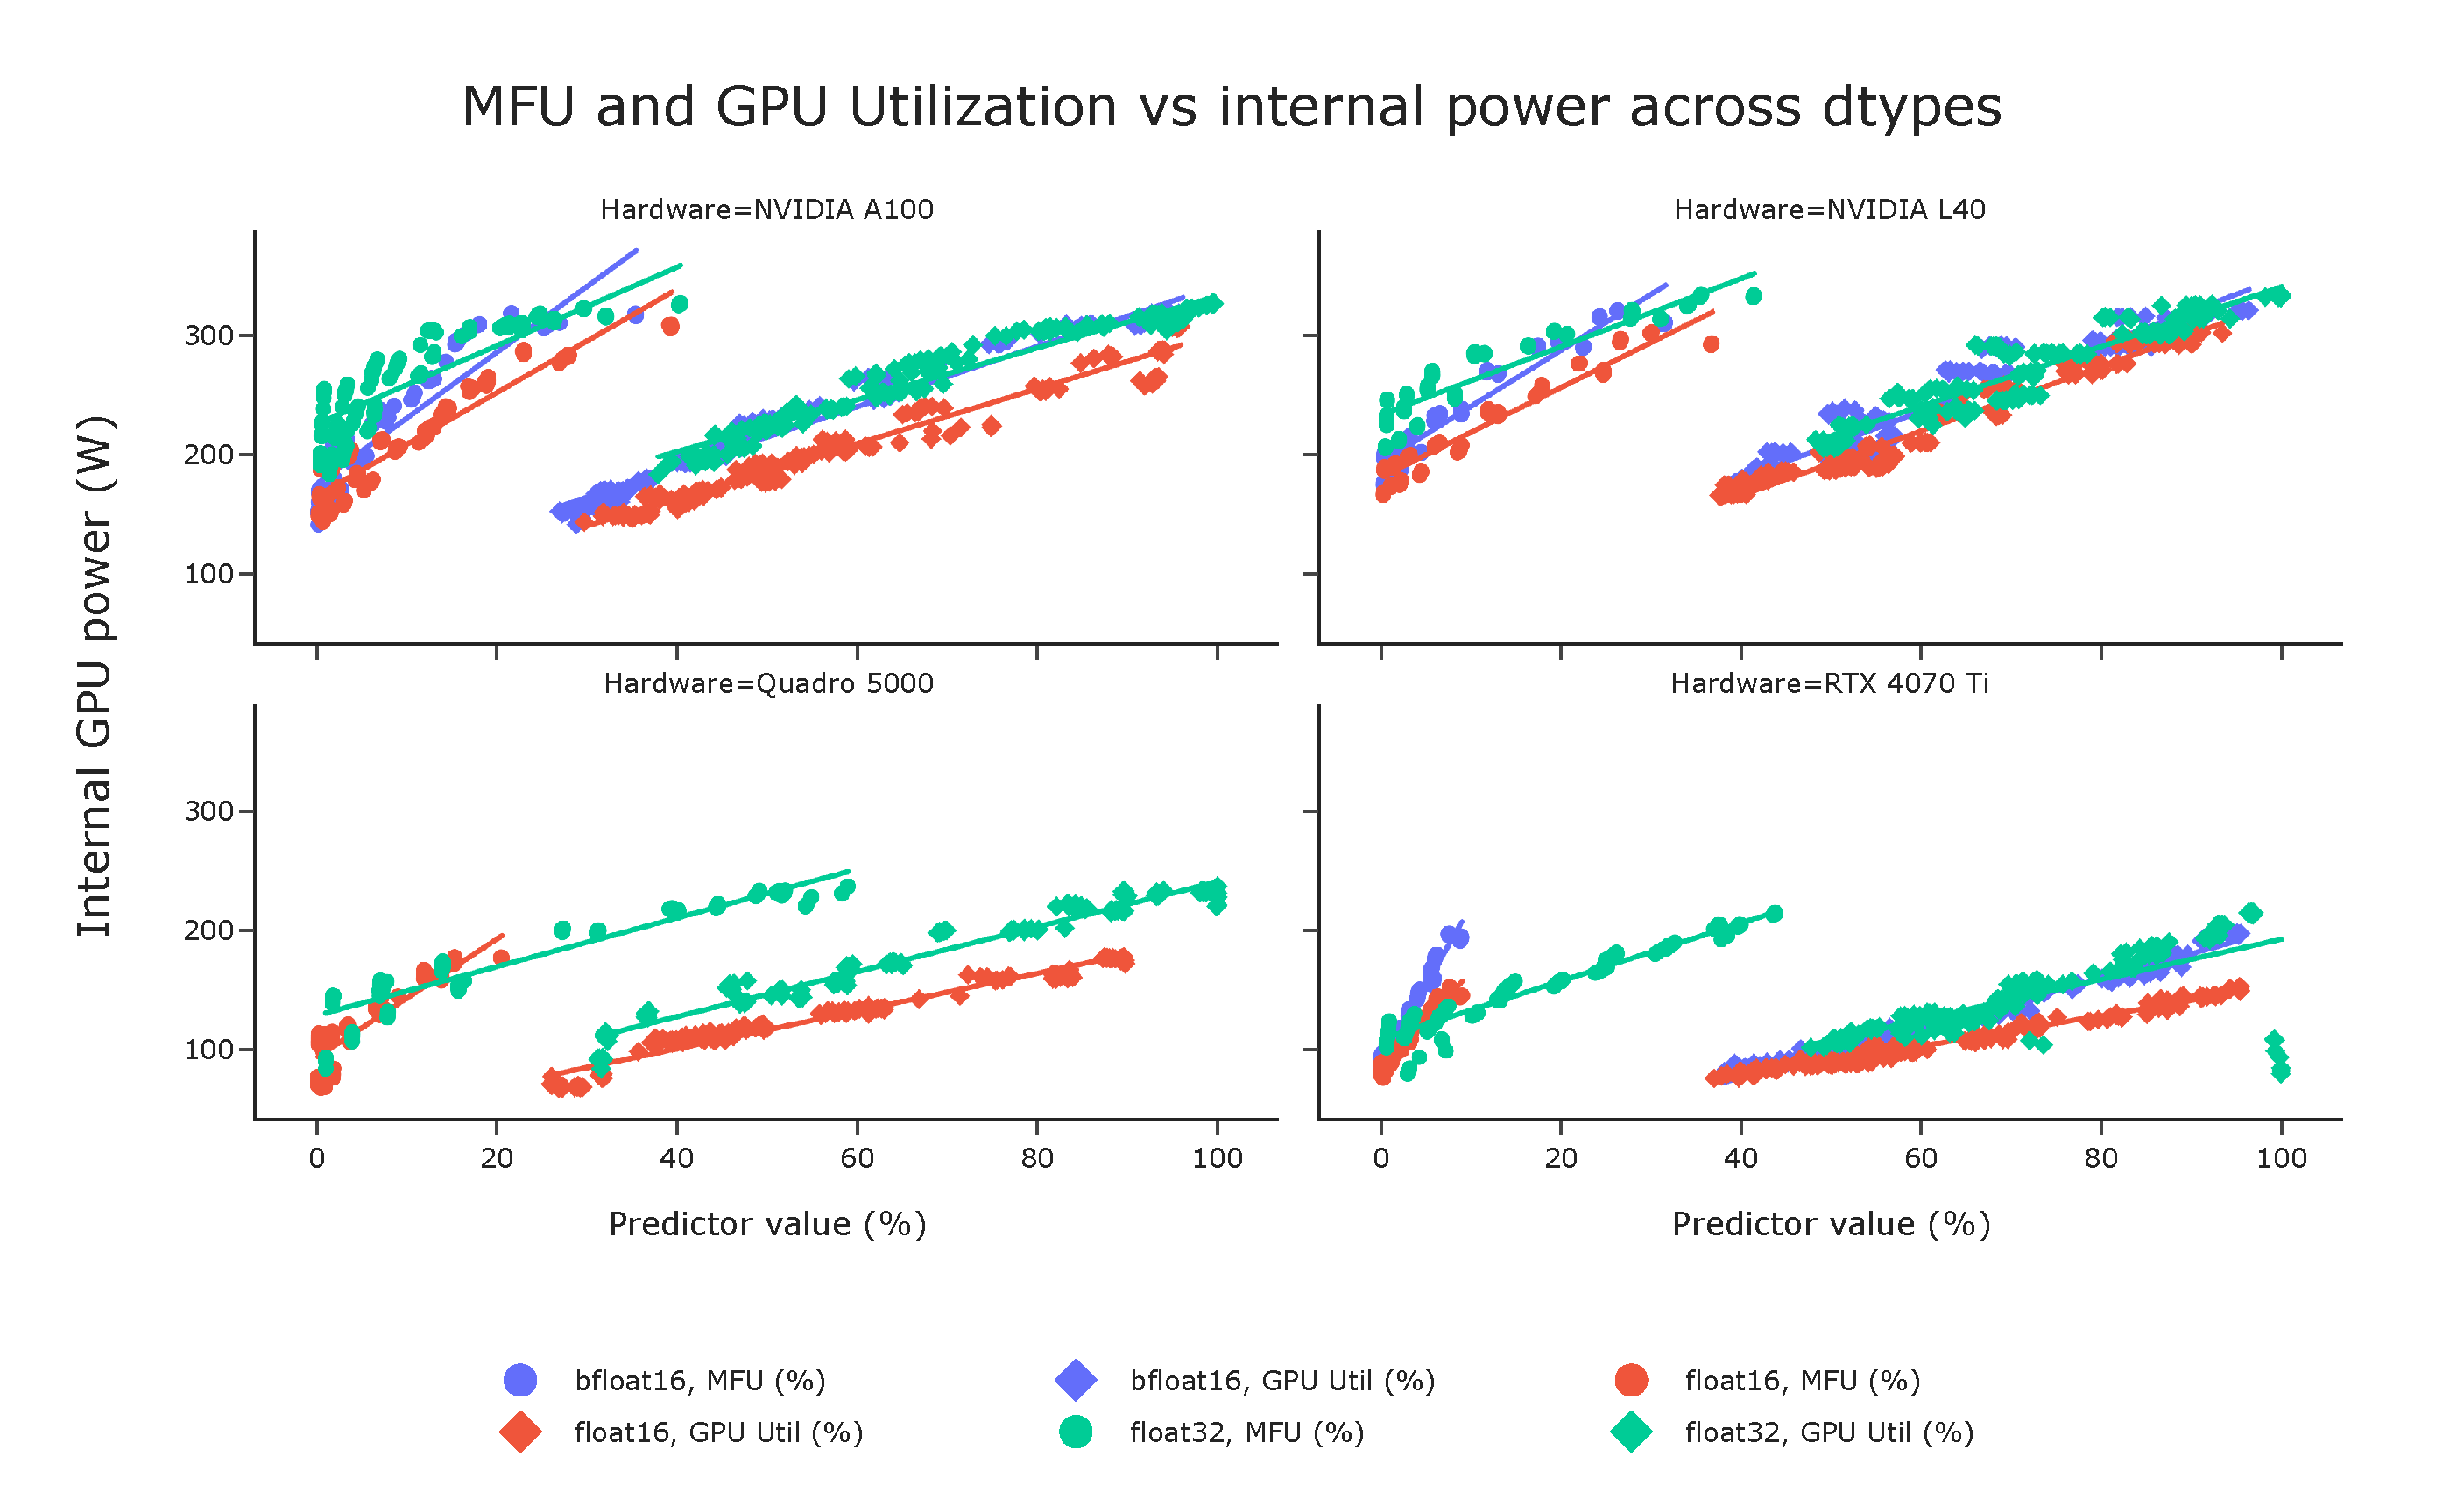
\includegraphics[width=\textwidth]{Figures and Tables/Fig: MFU and GPU Utilization vs internal power across dtypes.pdf}
    \caption{Relationship between MFU, GPU Utilization, and internal GPU power across numerical precisions. - }
    \label{fig:Predictors across DTypes}
\end{figure}

The analysis of context window size (512 vs 2048 tokens) shows no meaningful effect on predictor distributions. Median values, variance and overall spread remain nearly identical across all devices, with numerical differences below one percentage point. Warmup iterations and cooldown phases likewise exhibit only negligible effects on both predictors, with very low $R^2$ values and consistent trends across hardware. These parameters therefore do not influence steady-state predictor values within the evaluated range. 

Batch size, in contrast, introduces a pronounced and monotonic change in both predictors across all hardware platforms. Increasing the batch size from 1 to 128 leads to a substantial absolute change in GPU Util., reaching up to 53.5\% on the NVIDIA A100, and 34.7\% in MFU on the Quadro 5000. This behavior is further reflected by the consistently positive slopes per batch and the corresponding coefficients of determination that indicate a strong positive relationship between batch size, MFU and GPU Util.. This behavior was to be expected, as an increase in batch size typically leads to an increase of parallel compute work issued by the kernel. A logical conclusion is a rising value for performance based metrics.

A key observation is that numerical precision and batch size introduce systematic and pronounced changes in both predictors, whereas context window size, warmup iterations, and cooldown phases do not. This distinction illustrates an important separation between variables that directly influence execution performance, and those that affect workload structure without altering GPU steady-state behavior. 

In the context of energy modeling, these findings imply that behavior is robust across operational parameters that do not alter compute saturation. However, the impact of experimental variables must be interpreted with the two different evaluation regimes in mind, established in this thesis. Within individual, fixed configurations, MFU tends to reflect small variations in power consumption more sensitively. Across aggregated samples, GPU Util. becomes the more consistent predictor due to its broader capture of device activity. Consequently, MFU-based power estimations remain meaningful when execution characteristics are well controlled and homogeneous, while cross-configuration modeling benefits more strongly from GPU Util.. The increased sensitivity of MFU to dtype effects highlights the importance of acknowledging workload configurations when interpreting MFU-based predictions in heterogeneous settings.


%###############################################################################

\section{Limitations}\label{Limitations}
While the experimental design of this study enables consistent comparisons across predictors of and hardware platforms, several limitations constrain the generalizability of the findings.

External hardware power meters were only accessible for the NVIDIA Quadro 5000 and the L40, while the A100 and RTX 4070 Ti were evaluated using only software-reported values. Although the externally validated devices exhibited strong and stable linear relationships between internal GPU-reported power and the broader node-level measurements, the absence of real external validation for half of the analyzed hardware telemetry prevents an absolute accuracy assessment. 
The study also evaluates mostly NVIDIA GPUs, spanning from consumer-level to data-center-level accelerators. This selection provides a meaningful contrast in architectural tier and deployment setting, but does not capture behavior across multiple accelerator generations or system designs with substantially different power management policies. Results therefore may not generalize to other accelerators with different workload behavior.
Additionally, the RTX 4070 Ti was measured in a workstation environment, rather than in a dedicated compute node, which introduced uncontrolled background activity and runtime interference. While this setup provides a realistic depiction of consumer-grade deployment conditions, it increases result variability and may reduce comparability with more controlled systems.

%###############################################################################

\section{Conclusion}\label{Conclusion}
This work evaluated MFU and GPU Util. as predictors of GPU power consumption for generative AI workloads across four NVIDIA accelerators. Both metrics showed a clear and approximately linear relationship with internal GPU power, confirmed by external validation where available. When aggregating heterogeneous configurations, GPU Utilization remained the more robust single predictor, exhibiting higher explained variance and lower worst-case errors. In contrast, MFU consistently outperformed GPU Utilization within fixed, compute-bound configurations, where throughput dominates runtime behavior.

These results highlight that the relative usefulness of both metrics is inherently context-dependent. GPU Utilization is preferable in diverse or unstable execution regimes, while MFU offers stronger predictive accuracy when configurations are controlled and compute saturation is stable. Importantly, because MFU derives from high-level execution properties rather than hardware telemetry, it provides a practical and portable alternative for analytical models, simulators, and performance studies where GPU Utilization is unavailable. Together, these findings demonstrate that MFU enables hardware-agnostic power estimation while preserving meaningful alignment with measured energy behavior.

%###############################################################################

\bibliographystyle{splncs04}
\bibliography{sources}


\end{document}
